\documentclass[12pt, twoside]{article}
\usepackage[utf8]{inputenc}
\usepackage[english,russian]{babel}
\newcommand{\hdir}{.}

\usepackage{graphicx}
\usepackage{caption}
\usepackage{amssymb}
\usepackage{mathrsfs}
\usepackage{euscript}
\usepackage{upgreek}
\usepackage{array}
\usepackage{theorem}
\usepackage{graphicx}
\usepackage{subfig}
\usepackage{caption}
\usepackage{color}
\usepackage{url}
\usepackage{amsmath, bm}

\usepackage{cancel}

\DeclareMathOperator*{\argmax}{arg\,max}
\DeclareMathOperator*{\argmin}{arg\,min}

\usepackage[left=2cm, right=2cm, top=3cm, bottom=3cm, bindingoffset=0cm]{geometry}

\newcommand{\Pb}{\mathcal{P}}

\setcounter{secnumdepth}{-1}

\begin{document} 

\title{Задание 3 по курсу "Байесовский выбор модели"}
\author{Грабовой Андрей, группа 574}
\date{}
\maketitle

\section{Задача 1}

По условию задачи:

$$p(\textbf{X}, \textbf{y}, \textbf{w}| \textbf{A}) = \prod_i N(\textbf{x}_i|\textbf{0}, \sigma^2 \textbf{I}_n)N(\textbf{w}|\textbf{0}, \textbf{A}^{-1})\prod_j p(y_j| \textbf{x}_j, \textbf{w}) , \eqno(1.1)$$
где $p(y_j = 1|\textbf{x}_j, \textbf{w}) = \frac{1}{1+\exp(-\textbf{w}^{\mathsf{T}}\textbf{x}_j)}$

Для простоты запишем (1.1) в следующем общем виде:

$$p(\textbf{X}, \textbf{y}, \textbf{w}| \textbf{A}) = p(\textbf{X})p(\textbf{w}|\textbf{A})p(\textbf{y}|\textbf{X},\textbf{w}). \eqno(1.2)$$

\paragraph{a)}
По формуле Байеса:
$$p(\textbf{w}|\textbf{X},\textbf{y},\textbf{A}) = \frac{p(\textbf{y}|\textbf{X},\textbf{w})p(\textbf{w}|\textbf{A})}{\int_{\textbf{w}'\in \mathbb{R}^{n}} p(\textbf{y}|\textbf{X},\textbf{w}')p(\textbf{w}'|\textbf{A}) d\textbf{w}'}= \frac{\mathcal{Q}(\textbf{w})}{\int_{\textbf{w}'\in \mathbb{R}^{n}} \mathcal{Q}(\textbf{w}')}, \eqno(1.3)$$
где введено обозначение $\mathcal{Q}(\textbf{w}) = p(\textbf{y}|\textbf{X},\textbf{w})p(\textbf{w}|\textbf{A})$.

Выполним аппроксимацию Лапласа:
$$\text{log}\mathcal{Q}(\textbf{w})\approx \text{log}\mathcal{Q}(\textbf{w}_\text{MAP}) + \cancel{\nabla  \text{log}\mathcal{Q}(\textbf{w}_\text{MAP})} + \frac{1}{2}(\textbf{w}-\textbf{w}_{\text{MAP}})^{\mathsf{T}}\nabla\nabla^{\mathsf{T}}  \text{log}\mathcal{Q}(\textbf{w}_\text{MAP})(\textbf{w}-\textbf{w}_{\text{MAP}})=$$
$$= \text{log}\mathcal{Q}(\textbf{w}_\text{MAP}) - \frac{1}{2}(\textbf{w}-\textbf{w}_{\text{MAP}})^{\mathsf{T}}\textbf{H}^{-1}(\textbf{w}-\textbf{w}_{\text{MAP}}), \eqno(1.4)$$
где введено обозначение $\textbf{H}^{-1} = -\nabla\nabla^{\mathsf{T}}  \text{log}\mathcal{Q}(\textbf{w}_\text{MAP})$.

Для нашей задачи найдем $\textbf{H}^{-1}$:
$$\textbf{H}^{-1} = -\nabla\nabla^{\mathsf{T}}(-\frac{1}{2}\textbf{w}^{\mathsf{T}}\textbf{A}^{-1}\textbf{w} - \textbf{1}^{\mathsf{T}}\log(1+\exp(-\textbf{X}^{\mathsf{T}}\textbf{w}))) =$$
$$= \textbf{A}^{-1} +\nabla\nabla^{\mathsf{T}}\textbf{1}^{\mathsf{T}}\log(1+\exp(-\textbf{X}^{\mathsf{T}}\textbf{w}))=$$
$$=  \textbf{A}^{-1} +\sum_{i=1}^{m} \nabla\nabla^{\mathsf{T}}\log(1+\exp(-\textbf{x}_i^{\mathsf{T}}\textbf{w}))=$$
$$=  \textbf{A}^{-1} +\sum_{i=1}^{m} \textbf{x}_i\textbf{x}_i^{\mathsf{T}}\frac{\exp(-\textbf{x}_i^{\mathsf{T}}\textbf{w})}{1+\exp(-\textbf{x}_i^{\mathsf{T}}\textbf{w})}-\textbf{x}_i\textbf{x}_i^{\mathsf{T}}\frac{\exp(-2\textbf{x}_i^{\mathsf{T}}\textbf{w})}{(1+\exp(-\textbf{x}_i^{\mathsf{T}}\textbf{w}))^2}. \eqno(1.5)$$

Тогда получаем:
$$\mathcal{Q}(\textbf{w}) \approx \mathcal{Q}(\textbf{w}_{\text{MAP}})\exp\left(-\frac{1}{2}(\textbf{w}-\textbf{w}_{\text{MAP}})^{\mathsf{T}}\textbf{H}^{-1}(\textbf{w}-\textbf{w}_{\text{MAP}})\right). \eqno(1.6)$$

Подставляя (1.6) в (1.3) получим:

$$p(\textbf{w}|\textbf{X},\textbf{y},\textbf{A}) \approx \frac{\mathcal{Q}(\textbf{w}_{\text{MAP}})\exp\left(-\frac{1}{2}(\textbf{w}-\textbf{w}_{\text{MAP}})^{\mathsf{T}}\textbf{H}^{-1}(\textbf{w}-\textbf{w}_{\text{MAP}})\right)}{\int_{\textbf{w}'\in \mathbb{R}^{n}} \mathcal{Q}(\textbf{w}_{\text{MAP}})\exp\left(-\frac{1}{2}(\textbf{w}'-\textbf{w}_{\text{MAP}})^{\mathsf{T}}\textbf{H}^{-1}(\textbf{w}'-\textbf{w}_{\text{MAP}})\right)d\textbf{w}'}=$$
$$= \frac{\exp\left(-\frac{1}{2}(\textbf{w}-\textbf{w}_{\text{MAP}})^{\mathsf{T}}\textbf{H}^{-1}(\textbf{w}-\textbf{w}_{\text{MAP}})\right)}{\int_{\textbf{w}'\in \mathbb{R}^{n}} \exp\left(-\frac{1}{2}(\textbf{w}'-\textbf{w}_{\text{MAP}})^{\mathsf{T}}\textbf{H}^{-1}(\textbf{w}'-\textbf{w}_{\text{MAP}})\right)d\textbf{w}'} = $$
$$ = N(\textbf{w}_{\text{MAP}}, \textbf{H}).\eqno(1.7)$$

Оценим $\textbf{w}_{\text{MAP}}$:
$$\textbf{w}_{\text{MAP}} = \argmax_{\textbf{w} \in \mathbb{R}^{n}} p(\textbf{w}|\textbf{X}, \textbf{y}, \textbf{A}) = \argmin_{\textbf{w} \in \mathbb{R}^{n}}\{-\log p(\textbf{y}|\textbf{X},\textbf{w}) - \log p(\textbf{w}|\textbf{A})\}, \eqno(1.8)$$
где $$p(\textbf{y}|\textbf{X}, \textbf{w}) = \prod_i \hat{p}_i^{y_i}(1-\hat{p}_i)^{1-y_i}; \quad -\log p(\textbf{w}|\textbf{A}) = \frac{1}{2}\textbf{w}^{\mathsf{T}}\textbf{A}^{-1}\textbf{w}; \quad\hat{\textbf{p}} = \frac{1}{1+\exp(-\textbf{X}^{\mathsf{T}}\textbf{w})}, \eqno(1.9)$$

Подставляя (1.9) в (1.8) получаем:
$$\textbf{w}_{\text{MAP}} = \argmin_{\textbf{w} \in \mathbb{R}^{n}}\{-\textbf{y}^{\mathsf{T}}\log \hat{\textbf{p}} - (1-\textbf{y})^{\mathsf{T}}\log (1-\hat{\textbf{p}}) +\frac{1}{2}\textbf{w}^{\mathsf{T}}\textbf{A}^{-1}\textbf{w}\}=$$
$$=\argmin_{\textbf{w} \in \mathbb{R}^{n}}\{
-\textbf{y}^{\mathsf{T}}\log \frac{1}{1+\exp(-\textbf{X}^{\mathsf{T}}\textbf{w})}
-(\textbf{1} - \textbf{y})^{\mathsf{T}}\log \frac{\exp(-\textbf{X}^{\mathsf{T}}\textbf{w})}{1+\exp(-\textbf{X}^{\mathsf{T}}\textbf{w})}
+\frac{1}{2}\textbf{w}^{\mathsf{T}}\textbf{A}^{-1}\textbf{w}\}\} = $$
$$=\argmin_{\textbf{w} \in \mathbb{R}^{n}}\{
(\textbf{1} - \textbf{y})^{\mathsf{T}}\textbf{X}^{\mathsf{T}}\textbf{w}
+\textbf{1}^{\mathsf{T}}\log(1+\exp(-\textbf{X}^{\mathsf{T}}\textbf{w}))
+\frac{1}{2}\textbf{w}^{\mathsf{T}}\textbf{A}^{-1}\textbf{w}\}, \eqno(1.10)$$
где введя обозначения $\mathcal{L}(\textbf{w}|\textbf{X},\textbf{y},\textbf{A}) =
(\textbf{1} - \textbf{y})^{\mathsf{T}}\textbf{X}^{\mathsf{T}}\textbf{w}
+\textbf{1}^{\mathsf{T}}\log(1+\exp(-\textbf{X}^{\mathsf{T}}\textbf{w}))
+\frac{1}{2}\textbf{w}^{\mathsf{T}}\textbf{A}^{-1}\textbf{w}$ получим следующую оптимизационую задачу для нахождения $\textbf{w}_{\text{MAP}}$:
$$\textbf{w}_{\text{MAP}} = \argmin_{\textbf{w} \in \mathbb{R}^{n}} \mathcal{L}(\textbf{w}|\textbf{X},\textbf{y},\textbf{A}). \eqno(1.11)$$

\begin{figure}[h!]\center
{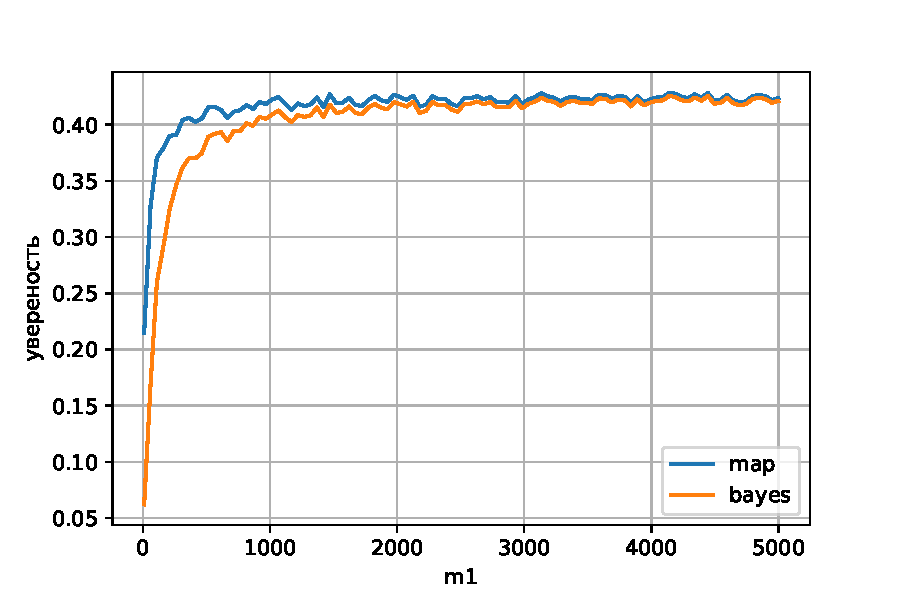
\includegraphics[width=0.8\textwidth]{Task1_1}}
\caption{График уверености, от размера обучающей выборки}
\label{Task1_1}
\end{figure}

\begin{figure}[h!]\center
\subfloat[m1=100]{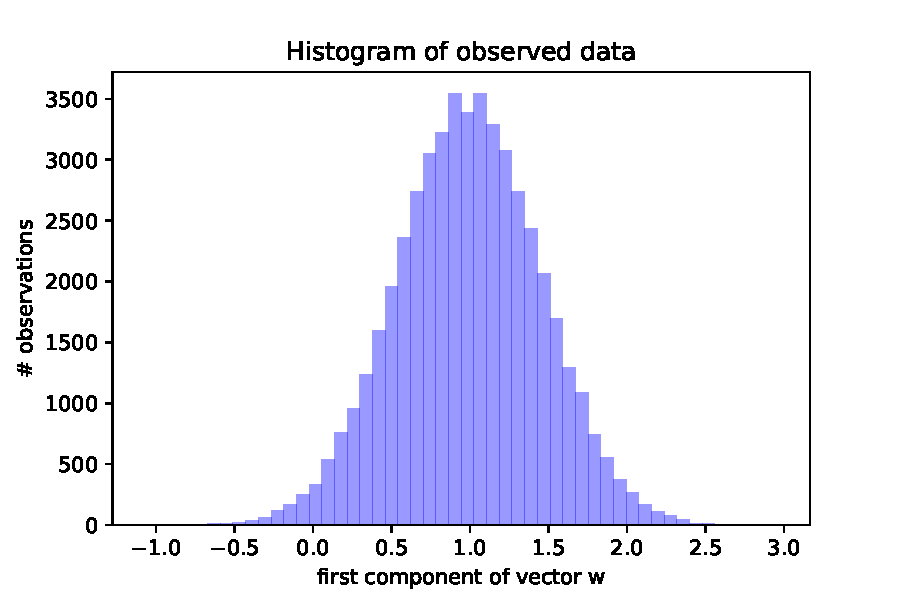
\includegraphics[width=0.5\textwidth]{Task1_3}}
\subfloat[m1=5000]{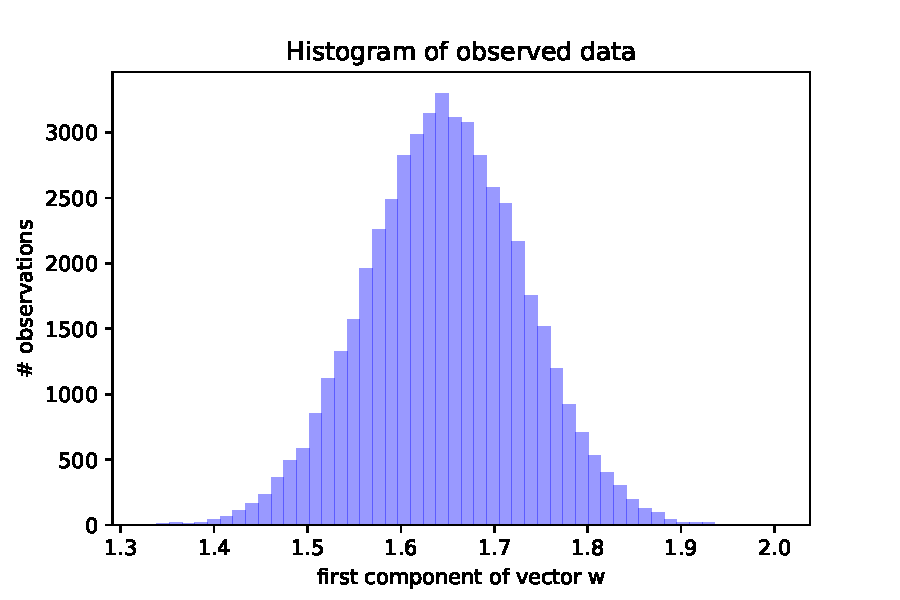
\includegraphics[width=0.5\textwidth]{Task1_4}}
\caption{Гистограмма распределения первой компоненты вектора $\textbf{w}\sim N(\textbf{w}_{\text{MAP}}, \textbf{H})$}
\label{Task1_3_4}
\end{figure}

\begin{figure}[h!]\center
{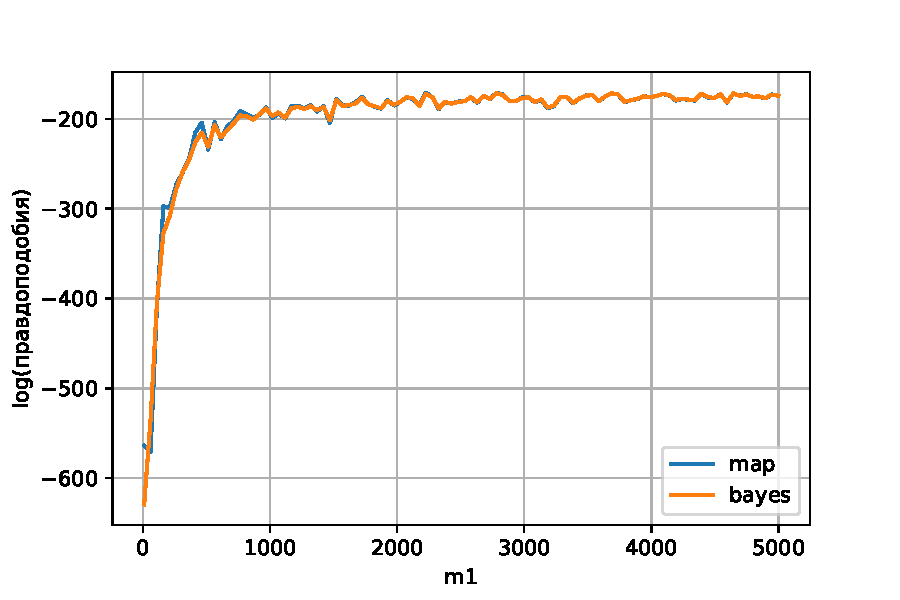
\includegraphics[width=0.8\textwidth]{Task1_2}}
\caption{График логарифма правдоподобия, от размера обучающей выборки}
\label{Task1_2}
\end{figure}

{\Large \textcolor{red}{Новая версия}}

\paragraph{b)} Пусть имеем следующии обучающие и тестовые выборки $(\textbf{X}_{train}, \textbf{y}_{train}) \in (\mathbb{R}^{m_1\times n}, \{0,1\}^{m_1})$ и $(\textbf{X}_{test}, \textbf{y}_{test}) \in (\mathbb{R}^{m_2\times n}, \{0,1\}^{m_2})$. Пусть $m_2=1000$, $\sigma^2 =1$, $\textbf{A} = \textbf{I}_n$, $n = 50$.

Пусть $\hat{\textbf{p}}$ --- вектор оценок вероятностей принадлежности объекта к клаасу 1 для некоторого классификатора на некоторой выборке $\textbf{X}$.

Введем уверенность $C(\hat{\textbf{p}})$ классификатора:
$$C(\hat{\textbf{p}}) = \sum_{i=1}^{m_2}|\hat{p}_i - 0.5|, \eqno(1.12)$$
где $m_2$ --- размер выборки.

Рассмотрим  правдоподобие выборки для заданого вектора $\hat{\textbf{p}}$ и истинных $\textbf{y}$:

$$l(\textbf{y}, \hat{\textbf{p}}) = \prod_{i=1}^{m_2}\hat{p}_i^{y_i}(1-\hat{p}_i)^{1-y_i}. \eqno(1.13)$$


Сравним уверенность и правдоподобие для точечного MAP-классификатора:
$$\hat{\textbf{p}}_{test}^{\text{MAP}} = \frac{1}{1+\exp(-\textbf{X}^{\mathsf{T}}\textbf{w}_{MAP})}, \eqno(1.14)$$
и для байесовского классификатора:
$$\hat{\textbf{p}}_{test}^{\text{BAYES}}  = \int_{\textbf{w}\in \mathbb{R}^{n}}\frac{p(\textbf{w}|\textbf{X}_{train}, \textbf{y}_{train}, \textbf{A})}{1+\exp(-\textbf{X}^{\mathsf{T}}\textbf{w})}d\textbf{w} =\mathsf{E}_{N(\textbf{w}_{\text{MAP}},\textbf{H})}\frac{1}{1+\exp(-\textbf{X}^{\mathsf{T}}\textbf{w})}. \eqno(1.15)$$

В виду что в формуле (1.15) сложный интеграл его будем считать сэмплированием (метод Монте Карло).
 
 Выборка генерировалась следующим образом. Сначала генерировался некоторый $\textbf{w}{\sim}N(\textbf{0},\textbf{A})$. После чего генерировалась выборка $\textbf{X}_{test}{\sim}N(\textbf{0},\sigma^2\textbf{I}_n)$ --- единая для всего эксперимента. После этого генерировался вектор ответов $\textbf{y}_{test} = \text{Be}\left(\frac{1}{1+\exp(-\textbf{X}^{\mathsf{T}}\textbf{w})}\right)$.   Далее для каждого $m_1$ генерировались выборки $\textbf{X}_{train},~\textbf{y}_{train}$.
 
 
На рис.~\ref{Task1_1} показано, что точечный MAP-классификатор является более уверенным в отличии от байесовского классификатору, что следует из того, что байесовский классификатор усредняет свой ответ. Важно заметить, что при увеличении размера выборки они ведут себя почти одинаково, это следует из того, что при большом количестве данных у нас становиться все более выраженный пик распределения. Изменения разброса значений $\textbf{w}$ показано на рис.~\ref{Task1_3_4}. Видно, что при $m_1 = 100$ разброс в первой компоненте намного больше чем разброс в первой компоненте при $m_1 = 5000$.


На рис.~\ref{Task1_2} показано, что байесовский классификатор и MAP-классификатор дают более менее одинаковое правдоподобие модели.

Из описанного выше можно сделать вывод, что байесовский классификатор является более устойчивым и при большом количестве данных он сходиться к распределению который имеет пик в матожидание, если этот вектор хорошо описывает выборку.

\section{Задача 2}
Пусть имеется модель линейной регрессии:
$$\textbf{y} = \textbf{X}\textbf{w} + \bm{\varepsilon}, \quad \bm{\varepsilon}{\sim}N(\textbf{0}, \sigma^2\textbf{I}), \eqno(2.1)$$
где $\sigma^2$ --- задано, и задано априорное распределение $p(\textbf{w}| \textbf{m}, \text{diag}(\textbf{s}))$.

Из (2.1) получаем распределение на $p(\textbf{y}, \textbf{w}|\textbf{X}, \textbf{m}, \textbf{s})$:
$$p(\textbf{y}, \textbf{w}|\textbf{X}, \textbf{m}, \textbf{s})) = p(\textbf{y}|\textbf{X}, \textbf{w})p(\textbf{w}|\textbf{m},\textbf{s}) = N(\textbf{Xw}, \sigma^2\textbf{I}) N(\textbf{m}, \text{diag}(\textbf{s})). \eqno(2.2)$$

Тогда по формуле Байеса получаем апостериорное распределение на вектор $\textbf{w}$:
$$p(\textbf{w}|\textbf{X}, \textbf{y}, \textbf{m}, \textbf{s}) = \frac{p(\textbf{y},\textbf{w}|\textbf{X}, \textbf{m}, \textbf{s})}{p(\textbf{y}|\textbf{X},\textbf{m},\textbf{s})} = \frac{p(\textbf{y}|\textbf{X}, \textbf{w})p(\textbf{w}|\textbf{m},\textbf{s})}{\int_{\textbf{w}'\in \mathbb{R}^{n}} p(\textbf{y},\textbf{w}'|\textbf{X}, \textbf{m}, \textbf{s})d\textbf{w}'} = \frac{\mathcal{Q}(\textbf{w})}{\int_{\textbf{w}'\in \mathbb{R}^{n}} \mathcal{Q}(\textbf{w}')d\textbf{w}'}, \eqno(2.3)$$
где введено обозначение $\mathcal{Q}(\textbf{w}) = p(\textbf{y}|\textbf{X}, \textbf{w})p(\textbf{w}|\textbf{m},\textbf{s})$.

Найдем $\textbf{w}_{\text{MAP}}$:
$$\textbf{w}_{\text{MAP}} = \argmax_{\textbf{w} \in \mathbb{R}^n} \mathcal{Q}(\textbf{w}) = \argmin_{\textbf{w} \in \mathbb{R}^n} \frac{1}{2\sigma^2}(\textbf{y} - \textbf{X}\textbf{w})^{\mathsf{T}}(\textbf{y} - \textbf{X}\textbf{w}) + \frac{1}{2}(\textbf{w} - \textbf{m})^{\mathsf{T}}\textbf{A}^{-1}(\textbf{w} - \textbf{m}) =$$
$$= \argmin_{\textbf{w} \in \mathbb{R}^n} \mathcal{L}(\textbf{w}), \eqno(2.4)$$
$$ \frac{\partial \mathcal{L}}{\partial \textbf{w}^{\mathsf{T}}} = -\frac{1}{\sigma^2}\textbf{X}^{\mathsf{T}}(\textbf{y}-\textbf{X}\textbf{w}) + \textbf{A}^{-1}(\textbf{w}-\textbf{m}) =0 \Rightarrow$$
$$\Rightarrow -\frac{1}{\sigma^2}\textbf{X}^{\mathsf{T}}\textbf{y} + \left(\frac{1}{\sigma^2}\textbf{X}^{\mathsf{T}}\textbf{X} + \textbf{A}^{-1}\right)\textbf{w} - \textbf{A}^{-1}\textbf{m}=0\Rightarrow$$
$$\Rightarrow \textbf{w}_{\text{MAP}} = \left(\frac{1}{\sigma^2}\textbf{X}^{\mathsf{T}}\textbf{X} + \textbf{A}^{-1}\right)^{-1}\left(\frac{1}{\sigma^2}\textbf{X}^{\mathsf{T}}\textbf{y} + \textbf{A}^{-1}\textbf{m}\right), \eqno(2.5)$$
где $\textbf{A} = \text{diag}(\textbf{s})$

Найдем $\textbf{H}$:

$$\textbf{H} = \left(\nabla\nabla^{\mathsf{T}}\mathcal{L}\right)^{-1} = \left(\frac{1}{\sigma^2}\textbf{X}^{\mathsf{T}}\textbf{X} + \textbf{A}^{-1}\right)^{-1}, \eqno(2.6)$$



Получаем:

$$p(\textbf{w}|\textbf{X}, \textbf{y}, \textbf{m}, \textbf{s}) = N(\textbf{w}_{\text{MAP}}, \textbf{H}). \eqno(2.7)$$

Если некоторое $s_i = 0$, то как видно из формул (2.5) и (2.6) получим, что апостериорное распределение $i$-го элемента вектора равно константе $m_i$.

Если же воспользоваться свойством сопряженности, то получиться такие же параметры нормального распределения, я честно пересчитал, но сюда не стал вносить. Это достаточно очевидно, потому что на самом деле мы просто разложили квадратичную функцию до второго порядка, это мы и получили саму функцию. То есть в данном случае аппроксимация Лапласа дает точный ответ.

% {\Large \textcolor{blue}{Старое, как было раньше}}

% Промаксимизируем обоснованость по параметрам $\textbf{m}$ и $\textbf{s}$:
% $$\hat{\textbf{m}}, \hat{\textbf{s}} = \argmax_{\textbf{m}, \textbf{s} \in \mathbb{R}^n} \int_{\textbf{w}'\in \mathbb{R}^{n}} \mathcal{Q}(\textbf{w}')d\textbf{w}'. \eqno(2.8)$$

% С аппроксимации Лапласа для (2.8) получаем:
% $$\hat{\textbf{m}}, \hat{\textbf{s}} = \argmax_{\textbf{m}, \textbf{s} \in \mathbb{R}^n} (2\pi)^{\frac{n}{2}}\sqrt{\det\textbf{H}}\mathcal{Q}(\textbf{w}_{\text{MAP}}) = \argmax_{\textbf{m}, \textbf{s} \in \mathbb{R}^n} \mathcal{F}(\textbf{m}, \textbf{s}). \eqno(2.9)$$

% Тогда:


% $$\log\mathcal{F}(\textbf{m}, \textbf{s})= -\frac{1}{2}\left(\frac{1}{\sigma^2}||\textbf{y}-\textbf{X}\textbf{w}_{\text{MAP}}||^2 + \textbf{w}^{\mathsf{T}}_{\text{MAP}}\textbf{A}^{-1}\textbf{w}_{\text{MAP}}\right) -\frac{1}{2}\log\det\textbf{A} +\frac{1}{2}\log\det\textbf{H} + C. \eqno(2.10)$$

% Сначала минимизируем (2.10) по $\textbf{m}$, поэтому все слагаемые, которые не зависят от $\textbf{m}$ убираем:
% $$\log\mathcal{F}(\textbf{m}, \textbf{s}) = -\frac{1}{2}\left(\frac{1}{\sigma^2}\textbf{y}^{\mathsf{T}}\textbf{y}-2\textbf{w}^{\mathsf{T}}_{\text{MAP}}\textbf{X}^{\mathsf{T}}\textbf{y} + \textbf{w}^{\mathsf{T}}_{\text{MAP}}(\textbf{A}^{-1} + \frac{1}{\sigma^2}\textbf{X}^{\mathsf{T}}\textbf{X})\textbf{w}_{\text{MAP}}\right) = $$
% $$= -\frac{1}{2\sigma^2}\textbf{y}^{\mathsf{T}}\textbf{y} +\frac{1}{\sigma^2}\left(\frac{1}{\sigma^2}\textbf{X}\textbf{y} +\textbf{A}^{-1}\textbf{m}\right)^{\mathsf{T}}\left(\frac{1}{\sigma^2}\textbf{X}^{\mathsf{T}}\textbf{X} + \textbf{A}^{-1}\right)^{-1}\textbf{X}^{\mathsf{T}}\textbf{y}-$$
% $$-\frac{1}{2}\left(\frac{1}{\sigma^2}\textbf{X}\textbf{y} + \textbf{A}^{-1}\textbf{m}\right)^{\mathsf{T}}\left(\frac{1}{\sigma^2}\textbf{X}^{\mathsf{T}}\textbf{X} + \textbf{A}^{-1}\right)^{-1}\left(\frac{1}{\sigma^2}\textbf{X}\textbf{y} + \textbf{A}^{-1}\textbf{m}\right) = $$
% $$=[\text{снова оставим только те слагаемые которые зависят от } \textbf{m}]=$$
% $$=-\frac{1}{\sigma^2}\textbf{m}^{\mathsf{T}}\textbf{A}^{-1}\left(\frac{1}{\sigma^2}\textbf{X}^{\mathsf{T}}\textbf{X} + \textbf{A}^{-1}\right)^{-1}\textbf{A}^{-1}\textbf{m}. \eqno(2.11)$$

% Как видно из (2.11) максимум достигается при $\textbf{m} = \textbf{0}$.

% Теперь минимизируем по $\textbf{s}$ с учетом того, что $\textbf{m} = \textbf{0}$:
% $$\log\mathcal{F}(\textbf{0}, \textbf{s}) = -\frac{1}{2}\left(\frac{1}{\sigma^2}\textbf{y}^{\mathsf{T}}\textbf{y}-2\textbf{w}^{\mathsf{T}}_{\text{MAP}}\textbf{X}^{\mathsf{T}}\textbf{y} + \textbf{w}^{\mathsf{T}}_{\text{MAP}}(\textbf{A}^{-1} + \frac{1}{\sigma^2}\textbf{X}^{\mathsf{T}}\textbf{X})\textbf{w}_{\text{MAP}}\right) -\frac{1}{2}\log\det \textbf{A} +\frac{1}{2}\log\det \textbf{H} =$$
% $$= -\frac{1}{2\sigma^2}\textbf{y}^{\mathsf{T}}\left(\textbf{I} - \frac{1}{\sigma^2}\textbf{X}\left(\frac{1}{\sigma^2}\textbf{X}^{\mathsf{T}}\textbf{X} + \textbf{A}^{-1}\right)^{-1}\textbf{X}^{\mathsf{T}}\right)\textbf{y} -\frac{1}{2}\log\det \textbf{A} +\frac{1}{2}\log\det \textbf{H} = $$
% $$=\left[\left(\textbf{I} - \frac{1}{\sigma^2}\textbf{X}\left(\frac{1}{\sigma^2}\textbf{X}^{\mathsf{T}}\textbf{X}+\textbf{A}^{-1}\right)^{-1}\textbf{X}^{\mathsf{T}}\right)^{-1} = \textbf{I} +\frac{1}{\sigma^2}\textbf{X}\textbf{A}\textbf{X}^{\mathsf{T}} \text{--- равенство Вудбери}\right]=$$
% $$=-\frac{1}{2\sigma^2}\textbf{y}^{\mathsf{T}}\left(\textbf{I} +\frac{1}{\sigma^2}\textbf{X}\textbf{A}\textbf{X}^{\mathsf{T}}\right)^{-1}\textbf{y} -\frac{1}{2}\log\det \textbf{A} +\frac{1}{2}\log\det \textbf{H} =$$
% $$=-\frac{1}{2\sigma^2}\textbf{y}^{\mathsf{T}}\left(\textbf{I} +\frac{1}{\sigma^2}\textbf{X}\textbf{A}\textbf{X}^{\mathsf{T}}\right)^{-1}\textbf{y} - \frac{1}{2}\log\left(\det\textbf{A}\det\left(\frac{1}{\sigma^2}\textbf{X}^{\mathsf{T}}\textbf{X} + \textbf{A}^{-1}\right)\right) = $$
% $$=\left[\det\left(\frac{1}{\sigma^2}\textbf{X}^{\mathsf{T}}\textbf{X} + \textbf{A}^{-1}\right) = \det\textbf{A}^{-1}\det\left(\textbf{I} +\frac{1}{\sigma^2}\textbf{X}\textbf{A}\textbf{X}^{\mathsf{T}}\right)\right] = $$
% $$= -\frac{1}{2\sigma^2}\textbf{y}^{\mathsf{T}}\left(\textbf{I} +\frac{1}{\sigma^2}\textbf{X}\textbf{A}\textbf{X}^{\mathsf{T}}\right)^{-1}\textbf{y} - \frac{1}{2}\log\det\left(\textbf{I} +\frac{1}{\sigma^2}\textbf{X}\textbf{A}\textbf{X}^{\mathsf{T}}\right). \eqno(2.12)$$

% Взяв производную от выражения (2.12) и прировняв к нулю, найдем значение вектора $\textbf{s}$.

% Из полученного результата можно сделать вывод, что лучше всего когда веса модели находятся в окрестности нуля.

{\Large \textcolor{red}{Новая версия}}
$$\hat{\textbf{m}}, \hat{\textbf{s}} =  \argmax_{\textbf{m}, \textbf{s} \in \mathbb{R}^n} \mathsf{E}_{N(\textbf{w}|\textbf{w}_{MAP}, \textbf{H})} \log p(\textbf{w}, \textbf{y}|\textbf{X}, \textbf{m}, \textbf{s}, \sigma) =  \argmax_{\textbf{m}, \textbf{s} \in \mathbb{R}^n} \mathcal{F}(\textbf{m}, \textbf{s}). \eqno(2.13)$$

Используя формулу (2.2) получаем:

$$\mathcal{F}(\textbf{m}, \textbf{s}) = \mathsf{E}_{N(\textbf{w}|\textbf{w}_{MAP}, \textbf{H})} \log \left(N(\textbf{y}|\textbf{X}\textbf{w}, \sigma^2\textbf{I})N(\textbf{w}|\textbf{m}, \textbf{s})\right)=$$
$$= \mathsf{E}_{N(\textbf{w}|\textbf{w}_{MAP}, \textbf{H})} \log N(\textbf{y}|\textbf{X}\textbf{w}, \sigma^2\textbf{I}) +  \mathsf{E}_{N(\textbf{w}|\textbf{w}_{MAP}, \textbf{H})}\log N(\textbf{w}|\textbf{m}, \textbf{s})=$$
$$= C-\frac{1}{2}\sum_{i=1}^{n}\log s_i - \frac{1}{2\sigma^2} \mathsf{E}_{N(\textbf{w}|\textbf{w}_{MAP}, \textbf{H})}||\textbf{y}-\textbf{X}\textbf{w}||^2 - \frac{1}{2}\mathsf{E}_{N(\textbf{w}|\textbf{w}_{MAP}, \textbf{H})}(\textbf{w} - \textbf{m})^{\mathsf{T}}\textbf{A}^{-1}(\textbf{w} - \textbf{m})=$$
$$= C-\frac{1}{2}\sum_{i=1}^{n}\log s_i - \frac{1}{2\sigma^2} \mathsf{E}_{N(\textbf{w}|\textbf{w}_{MAP}, \textbf{H})}||\textbf{y}-\textbf{X}\textbf{w}||^2  - \frac{1}{2} \sum_{i=1}^{n}\frac{ \mathsf{E}(w_i-m_i)^2}{s_i} . \eqno(2.14)$$

Если мы считаем, что на этом шаге у нас $\textbf{w}_{\text{MAP}}$ постоянная, тогда производная заносится под знак матожидания и мы получаем следующий результат:

$$\frac{\partial \mathcal{F}}{\partial \textbf{m}^{\mathsf{T}}} = \textbf{A}^{-1}\textbf{m} -  \mathsf{E}_{N(\textbf{w}|\textbf{w}_{MAP}, \textbf{H})} \textbf{A}^{-1}\textbf{w}=\textbf{0} \Rightarrow \textbf{m} =\textbf{w}_{\textbf{MAP}}, \eqno(2.15)$$

$$\frac{\partial \mathcal{F}}{\partial s_k} = -\frac{1}{2s_k} + \frac{1}{2s_k^2}\mathsf{E}_{{N(\textbf{w}|\textbf{m}, \textbf{H})}}\left(w_k- m_k\right)^2 = 0 \Rightarrow s_k = \mathsf{D}w_k. \eqno(2.16)$$

Из формул  (2.5) и (2.15) получаем:
$$\textbf{m} = \left(\frac{1}{\sigma^2}\textbf{X}^{\mathsf{T}}\textbf{X} + \textbf{A}^{-1}\right)^{-1}\left(\frac{1}{\sigma^2}\textbf{X}^{\mathsf{T}}\textbf{y} + \textbf{A}^{-1}\textbf{m}\right) \Rightarrow \textbf{m} = \left(\textbf{X}^{\mathsf{T}}\textbf{X}\right)^{-1}\textbf{X}^{\mathsf{T}}\textbf{y}, \eqno(2.17)$$
тоесть максимум обоснованности достигается, когда $\textbf{w}$ имеет распределение с матожиданием которое является решением уравнения $\textbf{y} = \textbf{X}\textbf{m}$ методом наименьших квадратов.

Из формул  (2.6) и (2.16) получаем:
$$\text{diag}(\textbf{A}) = \text{diag}\left[\left(\frac{1}{\sigma^2}\textbf{X}^{\mathsf{T}}\textbf{X} + \textbf{A}^{-1}\right)^{-1}\right], \eqno(2.18)$$
явно проитерировать это не смог, поэтому оставил в такой рекурентной формуле.

\section{Задача 3}
Пусть имеются две двухсторонние монеты, случайно и независимо выбранные из всех существующих монет достоинством в 2 рубля. Пусть было произведено $n_1 = 10$ бросаний первой монеты и $n_2 = 10000$ бросаний второй. Среди $n_1$ результатов бросания первой монеты было $k_1=3$ орла, а среди $n_2$ бросаний  второй --- $k_2=5050$ орлов.

% {\Large \textcolor{blue}{Старое, как было раньше}}
% \paragraph{a)}
% Пусть $k \in \mathbb{N}_0$ --- количество выпавших орлов, тогда имеем следующую вероятностную модель эксперимента: 

% $$p(k_1, p_1, k_2, p_2|n_1, n_2, \sigma) = q(p_1|\sigma)q(p_2|\sigma)\text{Bin}(k_1|p_1, n_1)\text{Bin}(k_2|p_2, n_2);$$
% $$
% q(p|\sigma)=\begin{cases} 
% \frac{N(p|\frac{1}{2}, \sigma^2)}{\int_0^1 N(x|\frac{1}{2}, \sigma^2)dx} & p \in [0,1]\\
% 0, & p \not\in [0,1]
% \end{cases}, \eqno(3.1)$$
% где  $q(p|\sigma)$ --- априорное распределение вероятности выпадении орла на монете. Априорное распределение вероятности задано таким образом, что бы математическое ожидание этой вероятности было $\frac{1}{2}$ и монотонно убывало в сторону увеличения и уменьшения. Это легко получить, если взять нормально распределение и для него исправить нормировочную константу так, как показано в формуле (3.1). Также был добавлен гиперпараметр $\sigma^2$ --- мера того насколько сильно мы сомневаемся в том что все монеты в мире имеют вероятность выпадения орла  $\frac{1}{2}$. Очевидно, что устремляя $\sigma$  в бесконечность получим, что все монеты равновероятные, а если устремить $\sigma$ к нулю то получим, что мы точно уверены, что все монеты симметричны.

% \paragraph{b)}

% \begin{figure}[h!]\center
% {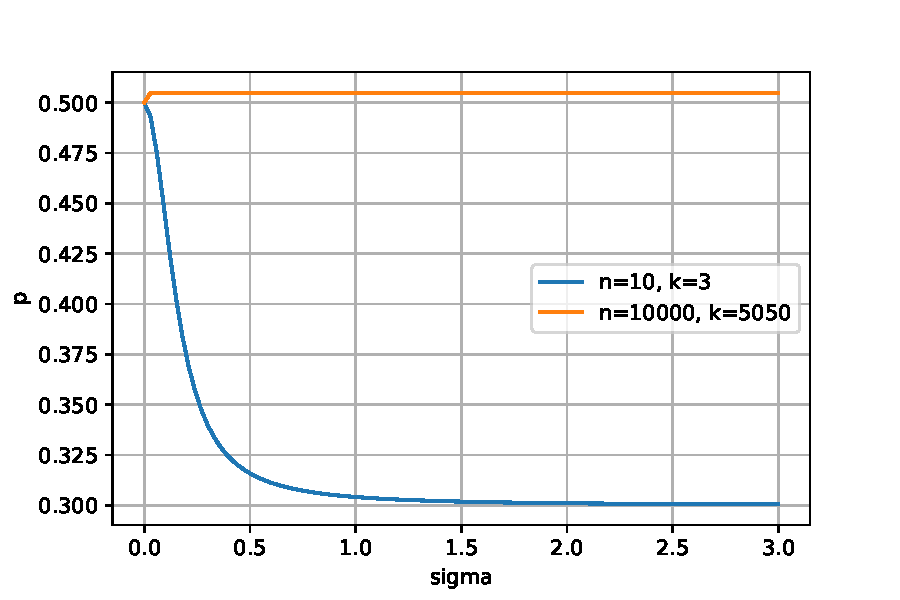
\includegraphics[width=0.8\textwidth]{Task3_1}}
% \caption{График $p_{\text{MAP}}$ в зависимости от $\sigma$}
% \label{Task3_1}
% \end{figure}

% По формуле Байеса получим апостериорное распределение $q(p|k,n,\sigma)$:
% $$q(p|k,n,\sigma) = \frac{p(k,p|n,\sigma)}{p(k|n, \sigma)}= \frac{p(k|p,n)q(p|\sigma)}{\int_0^1p(k|p',n)q(p'|\sigma)dp'} = \frac{\mathcal{Q}(p)}{\int_0^1 \mathcal{Q}(p')dp'}, \eqno(3.2)$$
% где $\mathcal{Q}(p) = p(k|p,n)q(p|\sigma)$.

% Для первого набора $n_1 =10, k_1 = 3$, используя аппроксимацию Лапласа, получаем:

% $$q(p_1|k_1,n_1, \sigma) =  N(p_1|p_1^{\text{MAP}}, h_1), \eqno(3.3)$$
% где  
% $$p_1^{\text{MAP}} = \argmax_{p \in [0,1]} \log \mathcal{Q}(p); \quad h_1 = - \left(\nabla\nabla^{\mathsf{T}}\log\mathcal{Q}(p)\right)^{-1}. \eqno(3.4)$$

% Найдем $p_1^{\text{MAP}}$:
% $$\frac{\partial \log\mathcal{Q}(p)}{\partial p} = \frac{k_1}{p}-\frac{n_1-k_1}{1-p}+\frac{\frac{1}{2}-p}{\sigma^2}=0\Rightarrow$$
% $$\Rightarrow p^3-\frac{3}{2}p^2+p(\frac{1}{2}-n_1\sigma^2)+k_1\sigma^2 = 0, \eqno(3.5)$$
% где $p_1^{\text{MAP}}$ решение уравнения (3.5). Аналитически решение найти не смог, но численно находиться решение легко. На рис.~\ref{Task3_1} показано как меняется $p_1^{\text{MAP}}$ в зависимости от гиперпараметра $\sigma$.

% Найдем $h_1$:
% $$h_1^{-1} = - \nabla\nabla^{\mathsf{T}}\mathcal{Q}(p) = -\frac{\partial^{2}\mathcal{Q}(p)}{\partial p^2} = \frac{k_1}{(p_1^{\text{MAP}})^2} + \frac{n_1-k_1}{(1-p_1^{\text{MAP}})^2} + \frac{1}{\sigma^2}, \eqno(3.6)$$

% Аналогично, для второго набора $n_2 =10000, k_2 = 5050$, используя аппроксимацию Лапласа, получаем:
% $$q(p_2|k_2,n_2, \sigma) =  N(p_2|p_2^{\text{MAP}}, h_2), \eqno(3.7)$$
% где $p_2^{\text{MAP}}$ находиться из решения уравнения (3.8), а $h_2$ задается уравнением (3.9):
% $$p^3-\frac{3}{2}p^2+p(\frac{1}{2}-n_2\sigma^2)+k_2\sigma^2 = 0. \eqno(3.8)$$
% $$h_2^{-1} =\frac{k_2}{(p_2^{\text{MAP}})^2} + \frac{n_2-k_2}{(1-p_2^{\text{MAP}})^2} + \frac{1}{\sigma^2}. \eqno(3.9)$$

% На рис.~\ref{Task3_1} показано, как меняется $p_2^{\text{MAP}}$ в зависимости от гиперпараметра $\sigma$.
% \paragraph{c)}
% Рассмотрим следующие модели $M_1$ и $M_2$:
% $$p_{M_1}(k_1, p_1, k_2, p_2|n_1, n_2, \sigma)=p_{M_1}(k_1, p, k_2|n_1, n_2, \sigma) = q^2(p|\sigma)\text{Bin}(k_1|p, n_1)\text{Bin}(k_2|p, n_2), \eqno(3.10)$$
% $$p_{M_2}(k_1, p_1, k_2, p_2|n_1, n_2, \sigma) = q(p_1|\sigma)q(p_2|\sigma)\text{Bin}(k_1|p_1, n_1)\text{Bin}(k_2|p_2, n_2), \eqno(3.11)$$
% где $p(M_1) = p(M_2) = \frac{1}{2}$.

% Тогда общая модель выглядит следующим образом:
% $$p(k_1, p_1, k_2, p_2, M_i|n_1, n_2, \sigma) = p(M_i)p_{M_i}(k_1, p_1, k_2, p_2|n_1, n_2, \sigma). \eqno(3.12)$$
% Найдем апостериорные вероятности моделей:
% $$p(M_i|k_1,n_1,k_2,n_2, \sigma) = \frac{p(M_i, k_1, k_2|n_1,n_2,\sigma)}{p(M_1, k_1, k_2|n_1,n_2,\sigma) + p(M_2, k_1, k_2|n_1,n_2,\sigma)}=$$
% $$= \frac{p(M_i)p_{M_i}(k_1,k_2|n_1,n_2,\sigma)}{p(M_1)p_{M_1}(k_1,k_2|n_1,n_2,\sigma)+p(M_2)p_{M_2}(k_1,k_2|n_1,n_2,\sigma)}. \eqno(3.13)$$

% Найдем $p_{M_1}(k_1, k_2|n_1,n_2,\sigma)$ и $p_{M_2}(k_1, k_2|n_1,n_2,\sigma)$:
% $$p_{M_1}(k_1, k_2|n_1,n_2,\sigma) = C\int_0^1 p^{k_1+k_2}(1-p)^{n_2+n_1-k_2-k_1}\exp\left(-\frac{(p-\frac{1}{2})^2}{\sigma^2}\right)dp, \eqno(3.14)$$
% $$p_{M_2}(k_1, k_2|n_1,n_2,\sigma) = C\int_0^1\int_0^1 p_1^{k_1}(1-p_1)^{n_1-k_1}p_2^{k_2}(1-p_2)^{n_2-k_2}\exp\left(-\frac{(p_1-\frac{1}{2})^2+(p_2-\frac{1}{2})^2}{2\sigma^2}\right)dp_1dp_2. \eqno(3.15)$$

% Посчитав это численно, получаем следующие апостериорные распределения на модели (считал при $\sigma = 1$):
% $$p(M_1) = 0.56;\quad p(M_2) = 0.44. \eqno(3.16)$$

% Как видно из (3.16) более простая модель $M_1$ имеет большую апостериорную вероятность, чем более сложная $M_2$.

{\Large \textcolor{red}{Новая версия}}
\paragraph{a)}
Пусть $k \in \mathbb{N}_0$ --- количество выпавших орлов, тогда имеем следующую вероятностную модель эксперимента: 

$$p(k_1, p_1, k_2, p_2|n_1, n_2) = q(p_1)q(p_2)\text{Bin}(k_1|p_1, n_1)\text{Bin}(k_2|p_2, n_2);$$
$$
q(p)=\begin{cases} 
1 & p \in [0,1]\\
0, & p \not\in [0,1]
\end{cases}, \eqno(3.17)$$
где  $q(p)$ --- априорное распределение вероятности выпадении орла на монете. Априорное распределение вероятности задано таким образом, что все монеты в мире равновероятны (теперь сделал так, чтобы потом интеграл хорошо брался, как-раз сразу видно сопряженное распределение).

\paragraph{b)}
По формуле Байеса получим апостериорное распределение $q(p|k,n)$:
$$q(p|k,n) = \frac{p(k,p|n)}{p(k|n)}= \frac{C_n^kp^{k}(1-p)^{n-k}}{\int_0^1C_n^kp'^{k}(1-p')^{n-k}dp'} = B(p|k+1, n-k+1), \eqno(3.18)$$
где $B(\alpha, \beta)$ --- бета распределение.

\paragraph{c)}
Рассмотрим следующие модели $M_1$ и $M_2$:
$$p_{M_1}(k_1, p_1, k_2, p_2|n_1, n_2)=p_{M_1}(k_1, p, k_2|n_1, n_2) = q(p)\text{Bin}(k_1|p, n_1)\text{Bin}(k_2|p, n_2), \eqno(3.19)$$
$$p_{M_2}(k_1, p_1, k_2, p_2|n_1, n_2) = q(p_1)q(p_2)\text{Bin}(k_1|p_1, n_1)\text{Bin}(k_2|p_2, n_2), \eqno(3.20)$$
где $p(M_1) = p(M_2) = \frac{1}{2}$.

Тогда общая модель выглядит следующим образом:
$$p(k_1, p_1, k_2, p_2, M_i|n_1, n_2) = p(M_i)p_{M_i}(k_1, p_1, k_2, p_2|n_1, n_2). \eqno(3.21)$$
Найдем апостериорные вероятности моделей:
$$p(M_i|k_1,n_1,k_2,n_2) = \frac{p(M_i, k_1, k_2|n_1,n_2)}{p(M_1, k_1, k_2|n_1,n_2) + p(M_2, k_1, k_2|n_1,n_2)}=$$
$$= \frac{p(M_i)p_{M_i}(k_1,k_2|n_1,n_2)}{p(M_1)p_{M_1}(k_1,k_2|n_1,n_2)+p(M_2)p_{M_2}(k_1,k_2|n_1,n_2)}. \eqno(3.22)$$

Найдем $p_{M_1}(k_1, k_2|n_1,n_2)$ и $p_{M_2}(k_1, k_2|n_1,n_2)$:
$$p_{M_1}(k_1, k_2|n_1,n_2) = C\int_0^1 p^{k_1+k_2}(1-p)^{n_2+n_1-k_2-k_1}dp, \eqno(3.23)$$
$$p_{M_2}(k_1, k_2|n_1,n_2) = C\int_0^1\int_0^1 p_1^{k_1}(1-p_1)^{n_1-k_1}p_2^{k_2}(1-p_2)^{n_2-k_2}dp_1dp_2. \eqno(3.24)$$

Получаем следующие апостериорные вероятности моделей:
$$p(M_1|k_1,n_1,k_2,n_2)  = \frac{Beta(\alpha_3, \beta_3)}{Beta(\alpha_3, \beta_3) + Beta(\alpha_1, \beta_1)Beta(\alpha_2, \beta_2)}, \eqno(3.25)$$
где $(\alpha_{1,2}, \beta_{1,2}) = (k_{1,2} + 1, n_{1,2}-k_{1,2} + 1)$; $(\alpha_{3}, \beta_{3}) = (k_{1}+k_{2} + 1, n_{1}+n_{2}-k_{1}-k_{2} + 1)$.

Посчитав, получаем следующие вероятности:
$$p(M_1|k_1,n_1,k_2,n_2) = 0.55, \qquad p(M_2|k_1,n_1,k_2,n_2) = 0.45.\eqno(3.26)$$

Снова таки, апостериорная вероятность более простой модели больше чем более сложной.

% \section{Задача 4}
% \paragraph{a)}
% KL - дивергенция это функция расстояния между распределениями $p(x)$ и $q(x)$ которая определяется следующим образом:
% $$KL(p||q) = \int p(x)\ln\frac{p(x)}{q(x)}dx. \eqno(4.1)$$
% Очевидно, что (4.1) не симметричная функция.

% Свойства KL-дивергенции:

% $$KL(p||q)\geq 0; \quad KL(p||q) = 0 \Leftrightarrow p\equiv q. \eqno(4.2)$$

% $$\text{Если } KL(p||q) < KL(q||p),\text{ то } p \text{ сильнее вложено в } q, \text{ чем } q\text{ в }p. \eqno(4.3)$$

% \paragraph{b)}
% Для доказательства воспользуемся неравенством Йенсена:
% $$f\left(\int\alpha(\textbf{x})y(\textbf{x}))d\textbf{x}\right) \geq \int\alpha(\textbf{x})f(y(\textbf{x}))d\textbf{x}, \eqno(4.4)$$
% Применив (4.4) получаем:
% $$0 = \log\left(\int p(x)\frac{q(x)}{p(x)}dx\right)\geq\int p(x)\log\frac{q(x)}{p(x)}dx=-KL(p||q), \eqno(4.5)$$

% \paragraph{c)}











\end{document} 